\chapter{Etat de l'art de l'ordonnancement et le  placement sur MC-NUMA} \label{chapter:opdag} 
%
Dans ce chapitre, Nous allons présenter l'état de l'art des problèmes d'ordonnance-ment des tâches et placement des données dans le contexte de NUMA en exposant les différentes approches proposées durant cette décennie. Comme nous l'avons montré, la plateforme NUMA donne une solution au problème de la scalabilité de la plateforme UMA mais en contre partie elle introduit la pénalité NUMA due aux accès distants générés par le placement des données d'une tâche sur un nœud différent du nœud sur lequel elle s'exécute. Ce facteur a un impact important sur le processus d'ordonnancement et il contribue à rendre le temps total d'exécution assez important pour un DAG par rapport  %celui d'
une exécution sur une plateforme UMA.
La figure suivante \ref{fig:FG_2_dag1006} montre un ordonnancement du mème DAG sur les plateformes UMA (un noeud de 8 coeurs N1C8) et NUMA (avec 4 noueds de 2 coeurs chacun N4C2) respectivement.
%
\begin{figure}
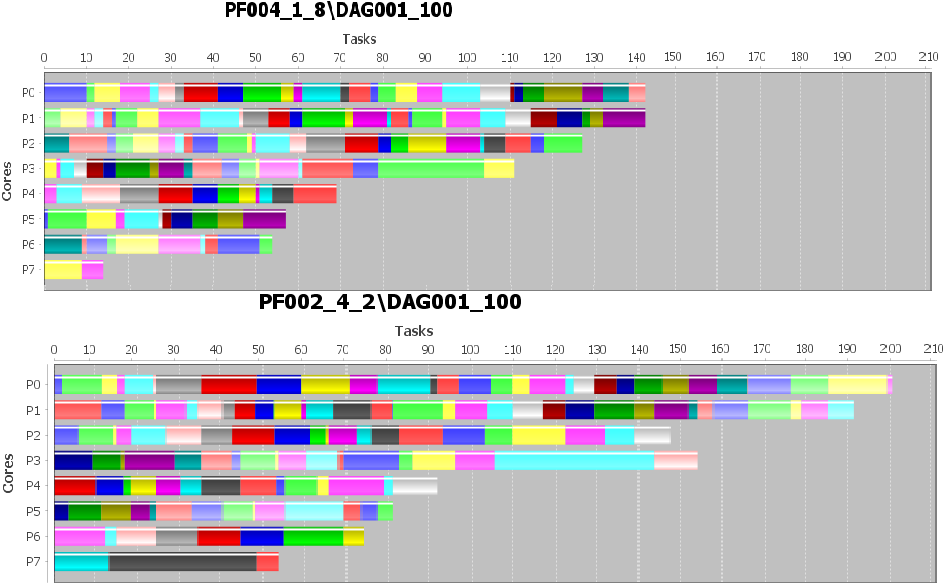
\includegraphics[scale=0.65]{dag1006}
\centering
\caption{Ordonnancement d'un DAG sur des plateformes UMA/NUMA}
\label{fig:FG_2_dag1006}
\end{figure}
%
Afin de réaliser l'objectif principal de l'ordonnancement et placement des données dans le contexte NUMA, les approches conçues ont été basé sur les idées qui exploitent certaines caractéristiques des architectures cibles \cite{Dreb15},
dont les principales caractéristiques sont les suivantes: \\  
- Les caractéristiques des applications ciblées par l'approche (parallélisation des boucles ou application régulière, irrégulière). \\
- L'ensemble des heuristiques (ordonnancement uniquement, placement uniquement ou les deux combinés). \\
- Le support logiciel d'implémentation (Système d'exploitation, Système d'exécution, Compilateur, Bibliothèque, Application ou une combinaison). \\
- Les informations utilisées et comment elles sont obtenues (indications de placement, affinités de données obtenues par profilage, Annotation du code source, ..).\\
- Le modèle de programmation cible (processus indépendants, fork-join \cite{FJ11} ,  OpenMP \cite{Omp00} \cite{Omp01} \cite{Omp02} ou Cilk \cite{Cil00} \cite{Cil01}).

La programmation parallèle des tâches est une approche de plus en plus populaire pour répondre aux attentes en matière d'évolutivité, et de productivité pour les applications destinées à fonctionner sur des systèmes à plusieurs cœurs. 
Les performances de l'exécution d'un tel type de programme dépendent fortement d'un système d'exécution optimisé capable d'exploiter efficacement le matériel sous-jacent. 
L'optimisation pour la hiérarchie de la mémoire, (caches et l'accès à la mémoire non uniforme), est un facteur clé dans ce contexte 
qui peut être réalisée grâce à un ordonnance-ment optimisé des tâches sur les cœurs et à un placement optimisé des données sur les contrôleurs de mémoire.   
Elle doit s'adapter à l'évolution rapide des architectures (nombre croissant des unités de calcul, réseaux d'interconnexion compliqué) et réagir aux changements dynamiques du comportement de l'application au moment de l'exécution pour équilibrer la charge.
Les approches peuvent être divisées en trois groupes \cite{Dreb15}\\
1- Aides à la prise de décision dont les informations sur les données pertinentes doivent être fournies par le programmeur.\\
2- Automatisant la prise de décision dont les informations fournies par le programmeur.\\
3- Automatisant la prise de décision et le recueil des informations sur les données pertinentes.

Les récents modèles de programmation parallèle à base de tâche tel que Cilk \cite{Cil00} \cite{Cil01}, OPENMP \cite{Omp00} \cite{Omp01} \cite{Omp02}, STARTS \cite{Sta00} et OPEN-STREAM \cite{Ost00} offrent de nouvelles opportunités au système d'exécution pour obtenir des informa-tions détaillées sur les données auxquelles accède une tâche ainsi que sur les dépendances inter-tâches. Ces modèles permettent de spécifier les dépendances inter-tâches en tant que dépendances de données et 
ainsi fournir au système d'exécution des informations précises sur les accès aux données par chaque tâche et le partage de données entre les tâches.

Dans la section \ref{caracAppro}, Nous présentons les grandes lignes des approches proposées en donnant les aspects qui caractérisent chaque classe. 
Ensuite la section \ref{ordoTKs} expose la première classe dont l'objectif principal est d'ordonnancer les tâches.
La deuxième classe qui focalise sur le placement est présentée dans la section \ref{placeDT}.
La section \ref{ordoPlaceComb} donne les approches qui combinent les deux aspects.
Comme l'équilibrage de charge est important pour préserver les performances, la section \ref{straECNUMA} est consacrée à détailler les stratégies utilisées pour cette fin.
Enfin la section \ref{concEdA} conclue le chapitre.\\
%=====================================================================================
\section{Caractéristiques des approches} \label{caracAppro}
L'étude des travaux connexes montre qu'il existe de nombreuses approches pour :\\ %différentes pour: \\
1- Améliorer la localisation des données par rapport à NUMA.\\
2- Réduire les conflits sur les contrôleurs de mémoire et sur les réseaux d’interconnexion.\\
3- Améliorer l'exploitation des caches grâce à un ordonnancement et un placement des données optimisées.

Le but de cette section est de donner une synthèse des approches avant de les exposer et de mettre en évidence les différences entre elles. 
Cette synthèse est divisée en trois parties. \\
\textbf{La première} : fournit un aperçu des caractéristiques générales. \\
\textbf{La deuxième} : se concentre sur les fonctionnalités liées au placement de données optimisé\\
\textbf{La troisième} : résume les caractéristiques des approches basée sur l'ordonnancement
%
\subsection{Caractéristiques principales}
Les caractéristiques générales des approches peuvent être résumées comme suit: \\
- La \textbf{partie de la hiérarchie de mémoire} optimisée par l'approche, c'est-à-dire si elle vise à améliorer les accès à la mémoire principale ou aux caches.\\ 
- La \textbf{couche de mise en œuvre} de l'approche (\textbf{IMP}) (par exemple, une bibliothèque (\textbf{LB}), le système d'exploitation (\textbf{OS}) ou le compilateur (\textbf{CP})).\\ 
- L'\textbf{infrastructure prise en charge} pour le parallélisme (par exemple, OpenMP, threads POSIX ou Cilk). \\
- La \textbf{technique} (\textbf{TCH}) sur laquelle est basée l'approche(sur un ordonnancement optimisée (\textbf{S}), un placement de données optimisé (\textbf{P}) ou si elle combine les deux techniques (\textbf{C})). 
%
\subsection{Caractéristiques du placement de données}
Les approches qui prennent en charge le placement de données diffèrent en ce qui concerne: \\
- \textbf{Source des données pertinentes SDP} : comment elles déterminent quelles données sont pertinentes pour améliorer le placement de données, en particulier si cela est fait automatiquement \textbf{A} ou si le programmeur \textbf{P} doit spécifier des structures de données pertinentes. \\
- \textbf{Les types de structures de données TSD} : quels types de structures de données sont supportés (par exemple, des tableaux ou toute région mémoire contiguë). \\
- \textbf{La granularité GRN} pour le placement de données (des éléments de données uniques, des pages ou des blocs représentant de grandes régions de mémoire). \\
- \textbf{Le moment de décision ToP} de placement est prise (par exemple, dynamiquement au moment de l'exécution, de manière statique au moment de la compilation ou pendant le profilage hors ligne). \\
%
\subsection{Caractéristiques des mécanismes d'ordonnancement}
Pour distinguer les approches de l'ordonnancement, nous avons identifié les caracté-ristiques suivantes: \\
- \textbf{Le type TYP} (par exemple, verrouillage de thread simple \textbf{THD}, ordonnancement de boucle \textbf{LOOP}). \\
- \textbf{La source des informations SID} sur lesquelles reposent les décisions (par exemple, les unités de surveillance des performances \textbf{SP}, les informations sur la distribution des données \textbf{DD} établies par l'approche elle-même ou le partage des données \textbf{SD} entre les threads).\\ 
- \textbf{Le type d'entités d'ordonnancement ENT} traitées par l'approche (par exemple, les threads du système d'exploitation, les itérations de boucle, les threads ou les tâches OpenMP). \\
- \textbf{Le moment de décision ToS} (par exemple, dynamiquement pendant l'exécution \textbf{EXE}, au début de l'exécution du programme \textbf{BEX} ou avant une boucle parallèle \textbf{BLP}).  
%=====================================================================================
\section{Ordonnancement des tâches}\label{ordoTKs}  %Scheduling and Mapping in MC-NUMA
%
Les approches suivantes reposent sur l'ordonnancement en tant que mécanisme princi-pal pour améliorer les performances des accès mémoire. 
\subsection{Principe de la réutilisation de l'ordonnancement}  
%
\textbf{1- Auteur}

Nikolopoulos et al. \cite{Nik01}.

\textbf{2- Idée}

Cette approche concerne la parallélisation des boucles. Elle prend en charge l'ordonnan-cement NUMA des itérations de boucle dans les applications OpenMP avec accès irrégulier à la mémoire principale. %Le premier exemple d'irrégularité géré par 
L'approche gère l'irrégularité des boucles imbriquées, où le bloc de l'itération de la boucle parallèle interne dépend de l'indice d'une boucle externe, de sorte que l'affectation des itérations de la boucle interne aux processeurs change entre itérations de la boucle externe. 
%
L'idée principale de l'approche est de distribuer d'abord les pages mémoires d'une structure de données accédée par une tâche (une boucle) sur des nœuds utilisant une description spécifique à l'application fournie par le programmeur par des annotations de code et de programmer des itérations des données sur les mêmes nœuds.
 
Le placement des pages est assuré par la politique first-touch qui place les pages de manière appropriée (sur le nœud de la première itération accédant à la structure de données). La localité de données est adressée en affectant des itérations suivantes accédant aux données aux processeurs associés aux nœuds contenant les données.

\textbf{3- Expérimentions}

La plateforme de l'expérimentation : c'est un système SGI Origin 2000 avec 64 proces-seurs regroupés en 32 nœuds.\\
Applications  :\\ 
1- \textbf{Décomposition de LU} (Application régulière), trois versions ont été comparé : \\
- une version OpenMP non modifiée. \\
- une version OpenMP modifiée avec des directives de distribution de données supportées par le compilateur SGI.\\
- l'approche SCHEDULE REUSE des auteurs.\\
\\
2- \textbf{Prévisions météorologiques} (Application irrégulière) deux variantes :\\
- Implémentés en utilisant OpenMP, avec l'approche SCHEDULE REUSE\\
- Avec le partitionnement de données explicite et le passage de message en utilisant MPI. 

\textbf{4-Evaluation}

L'approche de réutilisation de l'ordonnancement surpasse les deux versions d'Open-MP pour la décomposition de LU  
qu'elle surpasse les versions OpenMP non modifiées de l'Application de prévisions météorologiques et 
qu'elle offre des performances comparables aux Versions MPI.

\textbf{5- Commentaires}

La réutilisation de l'ordonnancement illustre que des informations statiques détail-lées sur les accès aux données, tirées du code source de l'application, peuvent être combinées avec une description d'une distribution de données spécifique à l'architecture pour une meilleure exploitation de la plateforme cible. 
%
\begin{center}%[htbp]
\begin{tabular}{l *{13}{l}} 		\hline
{TCH} & {IMP} 	& {SDP} 	&  {TSD} 	& {GRN} 	& {ToP} 	& {TYP} 	& {SPD}	& {ENT} 	& {ToS} \\     		\hline
C     	& CP+RT	& PRG		& ARY 	& ELT		& EXE		& LOOP	& DD 	  	& ITR 		& EXE    \\     		          \hline
\end{tabular}
 \captionof{table}{Caractéristiques de l'approche réutilisation de l'ordonnancement}% Add 'table' caption
\end{center} 
%
\subsection{Ordonnancement du parallélisme non structuré}\label{ordoPNS}
%
\textbf{1- Auteur}

Yoo et al. dans \cite{Yoo86}.

\textbf{2- Idée}

Le but de cette approche est d'optimiser les applications avec un parallélisme non structuré (c'est-à-dire des sections parallèles avec des tâches indépendantes qui peuvent être ordonnancées dans n'importe quel ordre avec une possibilité de partage des données). 
Les auteurs se sont concentrés sur les performances du cache en exécutant des tâches qui partagent des données sur des cœurs proches dans la hiérarchie de la mémoire. 

L'approche comprend trois parties principales. \\
- La première partie, la \textbf{charge de travail est profilée} afin de dériver des informations sur le partage de données entre les tâches. \\
- La deuxième partie consiste à \textbf{grouper des tâches}, à classer des groupes et à affecter les groupes à des files d'attente de travail associées aux composants de la hiérarchie de mémoire. \\
- La troisième partie traite de l'\textbf{équilibrage dynamique de la charge} grâce à un détournement de tâche sensible à la localité. 

Le résultat de l'exécution du profilage est un graphe de partage de tâches dont les sommets représentent des tâches et dont les arcs non dirigés capturent les relations de partage de données entre les tâches. 
Le poids associé à une arête indique le nombre de lignes de cache accessibles par les deux tâches connectées par un arc. 
Le graphe est ensuite partitionné de manière heuristique et récursive en groupes pour chaque niveau de la hiérarchie de mémoire, en commençant par le cache de dernier niveau. 
Chaque groupe de tâches est choisi de sorte que l'ensemble de travail des tâches s'insère dans un cache du niveau ciblé dans la hiérarchie de mémoire et de sorte que le partage de données intra-groupe soit maximisé. 
Le résultat est une hiérarchie de groupes de tâches qui peuvent être ordonnancées sur les files d'attente associées à chaque composant de la hiérarchie de mémoire, 
%
Au moment de l'exécution, les tâches sont exécutées par des \textbf{threads de travail (worker)} avec un thread par cœur. 
Lorsqu'un thread (worker) a fini d'exécuter une tâche, il essaie d'abord d'obtenir une tâche de sa file d'attente locale associée à son cache de premier niveau.
Si cette file d'attente est vide, le worker tente de prendre des tâches de l'une des files d'attente associées au cache de premier niveau de ses cœurs voisins par rapport au niveau suivant dans la hiérarchie de mémoire. 
Si ces files d'attente sont également vides, le worker tente d'obtenir un groupe de tâches à partir de la file d'attente associée à son cache de deuxième niveau. 

\textbf{3- Expérimentation}

Cette approche a été appliquée sur les charges de travail générales (base de données, reconstruction d'image 3D, détection de collision, traitement d'image, multiplica-tion matricielle et solveur pour équations aux dérivées partielles).

\textbf{4- Evaluation}  

Le groupement de tâches, le classement et l'assignation aux files d'attente, mais sans vol de travail sensible à la localité, peuvent accélérer l'exécution de 2:39 sur 32 cœurs pour les tests de mémoire intensifs et jusqu'à 3:57 sur 1024 cœurs. 
Le vol de travail sensible à la localisation sur 32 cœurs peut accélérer l'exécution de 1:9 par rapport à un vol de travail aléatoire avec un déséquilibre de charge créé par un nombre de workers inférieur au nombre de cœurs. 

\textbf{5- Commentaires}

L'approche montre que l'exploitation du partage de données dans l'ordonnanceur peut conduire à des améliorations de performances significatives. 
Elle illustre également que l'affectation initiale des tâches peut être combinée avec une technique de vols de travail tenant compte de la localité pour l'équilibrage de charge qui réagit aux circonstances au moment de l'exécution. L’approche du parallélisme non structuré ne fournit aucune forme de placement de données explicite. 
%
\begin{center}%[htbp]
\begin{tabular}{l *{13}{l}} 		\hline
{TCH} & {IMP} 	& {SDP} 	&  {TSD} 	& {GRN} 	& {ToP} 	& {TYP} 	& {SPD}	& {ENT} 	& {ToS} \\     		\hline
S     	& RT		& -		& - 		& -		& EXE		& TASK	& DS 	  	& TASK 	& SoX    \\     		          \hline
\end{tabular}
 \captionof{table}{Caractéristiques de l'Ordonnancement du parallélisme non structuré}% Add 'table' caption
\end{center} 
%=====================================================================================
\section{Placement des données} \label{placeDT}
%
Dans cette section nous allons donner les différentes approches pour le placement des données.
%
\subsection{Affinity on touch AoT}
%
\textbf{1- Auteur}

L. Henrik et al. \cite{HEN000}, \cite{AffOnNextTouch}.

\textbf{2- Idée}

De nombreux systèmes d'exploitation utilisent le placement \textbf{AFFINITY-ON-FIRST -TOUCH (AoFT)} comme stratégie de placement par défaut, dans laquelle une \textit{page de mémoire physique est allouée sur le nœud associé à la tâche qui écrit en premier sur la page ou lit la page}. 
Si les cœurs qui initialisent les structures de données et ceux qui y accèdent se trouvent sur le même nœud, l'AoFT génère une forte densité d'accès mémoire local. 
Cependant, si les nœuds d'initialisation et les nœuds d'accès ne correspondent pas, cette stratégie peut entraîner un conflit élevé et une forte proportion d'accès à la mémoire distante.
 Une stratégie courante pour contourner ce problème consiste à \textit{migrer dynamiquement les pages après l'initialisation vers les nœuds qui effectuent les accès en écriture suivants}. 
Cette stratégie, appelée \textbf{AFFINITY-ON-NEXT-TOUCH (AoNT) ou MIGRATE-ON-NEXT-TOUCH}, peut être entièrement implémentée dans l'espace utilisateur en utilisant des appels système pour la protection mémoire et la migration de page synchrone ou dans l'espace noyau pour la migration transparente et asynchrone. 

\textbf{3- Expérimentation}

Löf et Holmgren \cite{HEN000} ont évalué une implémentation d'espace utilisateur de AoNT sur un domaine isolé de 8 nœuds d'un système Sun Fire 15000 exécutant une application calculant la diffusion d'ondes électromagnétiques dans un espace tridimensionnel principa-lement pour résoudre un ensemble d'équations en utilisant la méthode du gradient conjugué. Goglin et Furmento \cite{GF50} ont implémenté AoNT pour le noyau Linux sur un système AMD Opteron 8347HE à quatre nœuds.

\textbf{4- Evaluation}

En utilisant AoNT, la performance est améliorée jusqu'à 166\%, ce qui montre que le placement de données peut avoir un impact énorme sur les performances de l'application. 
Pour Goglin et Furmento \cite{GF50} ont comparé les performances à une implémentation d'espace utilisateur. 
L'implémentation basée sur le noyau est environ 30\% plus rapide et affiche un sur débit significativement moins important que l'implémentation de l'espace utilisateur pour les petites régions de mémoire. 

\textbf{5- Commentaires}

Les auteurs concluent qu'une implémentation de l'espace utilisateur est plus performan-te dans les cas où de plus grandes zones de mémoire connues par l'application doivent être migrées. 
L'implémentation d'espace noyau migre ces zones page par page, tandis qu'une implémentation d'espace utilisateur peut migrer chacune de ces zones en une seule opération avec une surcharge plus faible.
Cependant, il appartient au programmeur ou à un composant logiciel de niveau supérieur de déclencher la migration de la page. 
%
\begin{center}%[htbp]
\begin{tabular}{l *{13}{l}} 		\hline
{TCH} & {IMP} 	& {SDP} 	&  {TSD} 	& {GRN} 	& {ToP} 	& {TYP} 	& {SPD}	& {ENT} 	& {ToS} \\     		\hline
P     	& OS-LB	& PRG-PFL	& - 		& PG		& EXE		& - 	  	& - 		& -    		& -\\     		          \hline
\end{tabular}
 \captionof{table}{Caractéristiques de l'Affinity on Touch}
\end{center}
%
\subsection{CARREFOUR} 

\textbf{1- Auteur}

Dashti et. al \cite{Das44}.

\textbf{2- Idée}

C'est un mécanisme de placement de données compatible NUMA pour le noyau Linux.  
CARREFOUR essaie d'éviter la congestion sur les contrôleurs de mémoire et les liens d'interconnexion et 
considère la réduction de la latence des accès mémoire en améliorant la localisation des données uniquement comme objectif secondaire. 
L'approche est basée sur quatre techniques: \\
1- La \textbf{co-localisation de pages} : il place une page sur le même nœud que le cœur accédant\\
2- L'\textbf{entrelacement de pages} : il place les pages sur des nœuds de manière circulaire\\
3- La \textbf{réplication de page} : il réplique des pages sur plusieurs nœuds\\
4- Le \textbf{clustering co-programme} : il place les threads en fonction de leur intensité de partage de données. 

La combinaison de ces techniques et l'application de chaque technique dépendent du comportement des applications exécutées sur la machine. 
Cela implique \\
- des décisions globales qui activent ou désactivent des techniques individuelles globalement\\
- des décisions page-locales qui activent ou désactivent des techniques par page. \\
Les statistiques qui servent de base pour caractériser le comportement du programme sont dérivées des valeurs fournies par un composant de mesure qui utilise \textbf{INSTRUCTION-BASED SAMPLING (IBS)} \cite{IBS48}.

Les décisions globales sont prises en quatre étapes. Dans :

1- La première étape, le système décide si le placement de données est nécessaire ou non. 
À cette fin, CARREFOUR compare le nombre d'accès mémoire par unité de temps du système entier à un seuil déterminé expérimentalement de 50 accès par microseconde. 
Si la valeur réelle de l'application est inférieure au seuil, CARREFOUR est désactivé et aucune autre action n'est entreprise. 

2- La deuxième étape consiste à décider si la réplication de page doit être activée ou désactivée. 
Pour éviter une charge de synchronisation élevée en raison des mises à jour fréquentes du contenu des pages, la réplication de page est uniquement utilisée pour les applications dont la fraction d'accès en lecture à la mémoire DRAM est supérieure à 95\%. 

3- La troisième étape, CARREFOUR vérifie si l'entrelacement doit être utilisé pour distribuer les demandes à la mémoire principale à tous les contrôleurs de mémoire. 
Cette décision est basée sur le déséquilibre du contrôleur de mémoire, qui est défini comme l'écart-type de la fréquence des accès mémoire entre les nœuds. 
L'entrelacement n'est appliqué que si la valeur est supérieure à un seuil de 35\%. 

4- La co-localisation est activée pour les applications dont le taux d'accès local est inférieur à 80\%, c'est-à-dire que la fraction des accès mémoire qui cible un nœud local est inférieure à 80\%. 
Les décisions locales-locales sont prises individuellement pour chaque page en analysant les statistiques dérivées des échantillons IBS qui appartiennent aux instructions d'accès à la page. 
Une page est migrée vers un nœud si la migration de page est activée globalement et si la page n'est accessible que par les cœurs d'un seul nœud. 
La réplication de page se déclenche si le mécanisme est autorisé globalement et si la page n'a été consultée qu'en lisant les instructions.
Une page accessible par des cœurs de plusieurs nœuds en mode lecture et écriture est placée en utilisant le mécanisme d'entrelacement qui déplace la page sur le nœud avec le plus petit nombre d'accès mémoire par unité de temps afin de réduire les conflits. 

\textbf{3- Expérimentation}

L'évaluation expérimentale de CARREFOUR a été réalisée sur deux machines systèmes AMD Opteron à 16 et 24 cœurs respectivement, regroupées en quatre nœuds. 
Les applications utilisées pour cette évaluation sont la suite PARSEC BENCHMARK (version 2.1), le moteur de reconnaissance faciale FACEREC (version 5.0).
Les performances de CARREFOUR ont été comparées à la stratégie par défaut de mise en page de First-touch du noyau Linux, entrelacement sur tous les nœuds.

\textbf{5- Evaluation} 

CARREFOUR fonctionne nettement mieux que le placement de pages par défaut (jusqu'à 3:63 plus rapide). 
Comparé à l'entrelacement sur tous les nœuds, CARREFOUR améliore significativement la performance dans la plupart des cas et 
limite la dégradation des performances dans les cas où l'entrelacement entre tous les nœuds dégrade les perform-ances par rapport au positionnement par défaut du système d'exploitation. 

\textbf{5- Commentaires}

CARREFOUR ne parvient pas à améliorer les performances des applications avec des changements de comportement rapides en raison de la précision d'échantillonnage limitée nécessaire pour un échantillonnage à faible débit. 
CARREFOUR montre que la contention est un problème important sur les systèmes NUMA car les optimisations qui diminuent les contentions entraînent une amélioration significative du temps d'exécution. 
%
\begin{center}%[htbp]
\begin{tabular}{l *{13}{l}} 		\hline
{TCH} & {IMP} 	& {SDP} 	&  {TSD} 	& {GRN} 	& {ToP} 	& {TYP} 	& {SPD}	& {ENT} 	& {ToS} \\     		\hline
C     	& OS		& PFL		&  - 		& PG		& EXE		& THD CLS	& OS 		& OS THD  & EXE  \\     		          \hline
\end{tabular}
 \captionof{table}{Caractéristiques de l'approche CARREFOUR}% Add 'table' caption
\end{center}
%
\subsection{Interface memory affinity MAI}    %Thread pinning    	& -      		& PThreads    	& Start of execution      & -\\\lipsum 

\textbf{1- Auteur}

C. Pousa RibeiroDashti et. al \cite{MAI77}.

\textbf{2- Idée}

C' est une interface de placement de données dont l'implémentation fournit un certain nombre de politiques pour la distribution des pages d'un tableau:\\
1- \textbf{bind\_all} : place toutes les pages sur un seul nœud et ne passe pas à d'autres nœuds que si toute la mémoire du nœud actuel est en cours d'utilisation.\\
2- \textbf{bind\_block} : divise d'abord le tableau en blocs, puis place chaque bloc sur un nœud différent.\\ 
3- \textbf{cyclique} : distribue les pages d'un tableau de manière circulaire sur tous les nœuds de la machine, de telle sorte que la i$^{ième}$ page est placée sur le nœud dont l'identifiant est \textbf{i mod M}, \textbf{M} étant le nombre de nœuds. \\
4- \textbf{cyclic\_block} : distribue des blocs de pages suivantes sur des nœuds de manière circulaire.\\
5- \textbf{\_mapp} : combine deux politiques: d'abord, il associe des pages à $P$ blocs de données virtuels en utilisant la politique cyclique. La deuxième étape consiste à redistribuer les blocs virtuels aux nœuds en utilisant à nouveau la politique cyclique. \\
6- \textbf{random} : elle place les pages de manière aléatoire entre les nœuds. 

\textbf{3- Expérimentation}.

L'évaluation de MAI a été réalisée sur des systèmes à quatre et huit nœuds NUMA pour les applications FFT et CG de la version OpenMP du NAS PARALLEL BENCHMA-RKS ainsi que pour une implémentation OpenMP d'une application géophysique.

\textbf{4- Evaluation}. 

Les stratégies proposées par MAI peuvent améliorer les performances de jusqu'à 31\% par rapport à la stratégie d’AoFT par défaut du système d'exploitation, mais doivent être choisies manuellement. 

\textbf{5- Commentaires}

Les auteurs ont conclu que la meilleure stratégie pour le placement de données dépend de l'architecture cible ainsi que de la structure des accès mémoire. 
Les machines avec une grande différence entre la latence des accès locaux et distants bénéficient d'un placement de données optimisé pour la localité, comme bind\_block, 
tandis que l'exécution sur des machines avec une faible différence entre ces latences peut être améliorée avec un placement qui améliore la répartition cyclique, aléatoire. 
Les applications avec une affinité claire des calculs et des données donnent des performances plus élevées avec bind\_block et 
les applications avec des accès irréguliers bénéficient de la distribution des données sur les nœuds. 

Les résultats présentés dans l'évaluation expérimentale de MAI montrent que le compo-rtement d'une application nécessite différents types de distributions de données aux nœuds et souligne que l'architecture joue également un rôle important dans la sélection d'une stratégie de placement.
%
\begin{center}%[htbp]
\begin{tabular}{l *{13}{l}} 		\hline
{TCH} & {IMP} 	& {SDP} 	&  {TSD} 	& {GRN} 	& {ToP} 	& {TYP} 	& {SPD}	& {ENT} 	& {ToS} \\     		\hline
P     	& LB		& PRG		&  ARY 	& BL/PG	& EXE		& THD PIN	& - 		& PTH   	& SOX  \\     		          \hline
\end{tabular}
 \captionof{table}{Caractéristiques de l'approche MAI}% Add 'table' caption
\end{center}
%
\subsection{MINAS}

\textbf{1- Auteur}

C. Pousa RibeiroDashti et. al \cite{MINAS76}.

\textbf{2- Idée}

MINAS combine les capacités de placement de données de MAI avec un préproces-seur appelé MAPP et NUMARCH, un module qui fournit des informations sur l'architecture cible. 
MAPP traite le code source d'une application, trouve des tableaux statiques partagés et remplace leurs déclarations par des appels appropriés aux fonctions d'allocation et de distribution de mémoire de MAI. 
La politique réelle pour la distribution de données choisie par MAPP dépend des caractéristiques de la plate-forme NUMA signalée par NUMARCH. 
Pour les systèmes ayant une latence d'accès distant élevée par rapport à la latence des accès locaux, la politique bind\_block est choisie afin d'optimiser la latence. 
Sur les systèmes avec une latence d'accès à distance inférieure, le framework optimise la bande passante et utilise la politique cyclique. 

L'approche utilise deux métriques pour caractériser la communication : \\
1- la première est basée sur la quantité de mémoire accessible par deux threads \\
2- la seconde mesure le nombre d'accès aux blocs de mémoire partagée. 

\textbf{3- Expérimentation}.

L'évaluation expérimentale a été réalisée sur un système AMD Opteron 875 avec 8 nœuds NUMA et 16 cœurs au total, ainsi que sur un système Intel Xeon X7560 avec 4 nœuds NUMA et 32 cœurs au total. 
Les performances de l'optimisation automatique avec MINAS sont comparées à la politique de placement de pages par défaut du système d'exploitation ainsi qu'aux versions des applications réglées manuellement en utilisant des combinaisons de stratégies de distribution correspondant le mieux aux modèles d'accès aux données. 
Les applications utilisées pour l'évalua-tion sont les mêmes que pour l'évaluation de MAI avec un benchmark supplémentaire qui simule la propagation des ondes en trois dimensions. 
%Une autre évaluation où l'application est exécutée dans un simulateur de système complet ses accès mémoire sont enregistrés dans un fichier de trace qui sera analysé afin de générer des matrices de partage qui indiquent pour chaque paire de threads comment intensément ces threads communiquent.

\textbf{4- Evaluation}. 

La solution automatique améliore les performances par rapport à la stratégie de positionnement de page par défaut du système d'exploitation, mais reste derrière les performances des codes réglés manuellement. 
La différence entre les versions automatique et manuelle varie de 0\% à 25\%. 

Les auteurs ont montré que pour les mappages de threads et de données basés sur la matrice de partage, des améliorations significatives du temps d'exécution allant jusqu'à 75\% peuvent être réalisées par rapport au mappage de thread et de données par défaut du système d'exploitation. 

\textbf{5- Commentaires}

%Les résultats montrent que, 
Bien que l'approche automatique ne puisse pas correspondre aux performances du code réglé manuellement dans certain cas.
L'approche montre que le profilage peut être utilisé pour obtenir des informations détaillées sur les échanges de données entre threads, ce qui peut être exploité pour améliorer le positionnement des applications avec des modèles distincts pour les accès mémoire.
%
\begin{figure}[h]
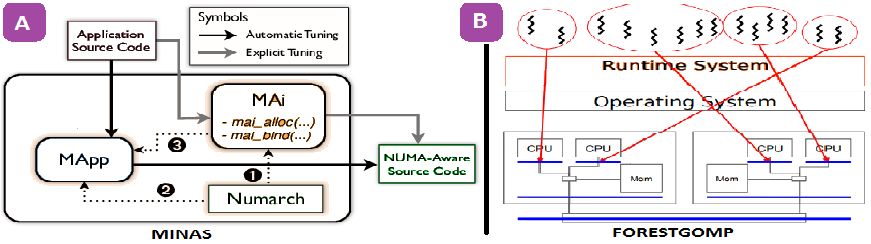
\includegraphics[scale=0.75]{Minas001}
\centering
\caption{MINAS Framework}
\label{fig:mci7}
\end{figure}   %\lipsum 
%
\begin{center}%[htbp]
\begin{tabular}{l *{13}{l}} 		\hline
{TCH} & {IMP} 	& {SDP} 	&  {TSD} 	& {GRN} 	& {ToP} 	& {TYP} 	& {SPD}	& {ENT} 	& {ToS} \\     		\hline
C     	& PP+LB	& PPR		&  ARY		& BL/PG	& EXE		& CoSCH	& DS 		& PTHD 	& SOX  \\     		          \hline
\end{tabular}
 \captionof{table}{Caractéristiques de l'approche MINAS}
\end{center}
%
\subsection{Placement de pages orienté feedback FBoPP}  % pour OpenMP FdP 
%
\textbf{1- Auteur}

Marathe et al \cite{Mar62}.

\textbf{2- Idée}

C'est un placement guidé par la trace de pages pour les programmes OpenMP. 
L'appro-che est divisée en trois phases:

a- \textbf{La génération de traces}\\
Pendant la génération de trace, le framework exécute une version tronquée du programme dont le placement de données doit être amélioré. 
il présente des informations détaillées sur les accès mémoire et les allocations de mémoire en utilisant les outils pour enregistrer les performances des processeurs et 
en interceptant les appels à l'allocateur de mémoire de la bibliothèque d'exécution C / FORTRAN. 

b- \textbf{La décision d'affinité}\\
Les décisions d'affinité consistent à déterminer sur quel nœud chaque page doit être placée, en fonction des accès de la trace. 
Le framework fournit un modèle simple, dans lequel la latence d'un accès à distance est supposée être indépendante de la distance entre le cœur demandeur et le nœud qui satisfait la demande. Dans ce modèle, une page est associée au nœud ayant le plus grand nombre d'accès à la page. Ainsi qu'un modèle plus sophistiqué qui prend en compte des latences variables. 

c- \textbf{Le placement de pages guidées par trace}\\
Le placement de page réel est effectué lors de l'exécution du programme entier en intercep-tant les appels à l'allocateur de mémoire et en initialisant des pages sur le nœud approprié avant de transmettre les régions de mémoire à l'application. 

\textbf{3- Expérimentation}\\
Les auteurs ont testé cette approche sur les applications de la version C du NAS PARALLEL BENCHMARKS et des applications des benchmarks SPEC OMPM2001 sur un système NUMA avec quatre nœuds.

\textbf{4- Evaluation}\\
le nombre d'accès mémoire distants et le temps d'exécution peut être diminué de manière significative . 

\textbf{5- Commentaires}\\
Le placement de pages orienté feedback est une approche qui exploite les informations obtenues par le biais du profilage pour améliorer le placement des données. 
%
\begin{center}%[htbp]
\begin{tabular}{l *{13}{l}} 		\hline
{TCH} & {IMP} 	& {SDP} 	&  {TSD} 	& {GRN} 	& {ToP} 	& {TYP} 	& {SPD}	& {ENT} 	& {ToS} \\     		\hline
C     	& OS		& PFL		&  - 		& PG		& EXE		& THD CLS	& OS 		& OS THD  & EXE  \\     		          \hline
\end{tabular}
 \captionof{table}{Caractéristiques de l'approche FBoPP}% Add 'table' caption
\end{center}
%==================================================================================
\section{Ordonnancement et placement combinés}\label{ordoPlaceComb}
%
Dans les sections suivantes, nous présentons les approches combinant l'ordonnan-cement et le placement dans le contexte NUMA.  
%
\subsection{FORESTGOMP} %Thread placement& Data distribution 	& OpenMP threads 	& Execution 	& x\\\lipsum

\textbf{1- Auteur}

Broquedis et al \cite{Bro29}.

\textbf{2- Idée}

FORESTGOMP est un runtime OpenMP avec un ordonnanceur ressource-aware basé sur l'ordonnanceur BUBBLESCHED \cite{BUB83} et un allocateur NUMA-aware basé sur l'interface mémoire MAMI \cite{MAM32}. 
il repose sur des indications précises sur les affinités entre les threads OpenMP et les données fournies par le programmeur. Il est basé sur trois concepts clés :

1- \textit{Le regroupement des threads OpenMP en bulles}.\\
a- Extraction automatiquement les informations sur la hiérarchie de la mémoire de la plateforme cible à l'aide de HWLOC \cite{HWL30} \\
b- Création d'une hiérarchie de files d'attente reflétant cette topologie.
le système d'exécu-tion peut créer une file d'attente pour l'ensemble de la machine, une file d'attente pour chaque nœud NUMA, une file d'attente pour chaque cache partagé et une file d'attente pour chaque cœur. 
Chacune des files d'attente d'exécution forme un domaine d'ordonnan-cement qui limite l'exécution des entités d'ordonnancement dans la file d'attente à la partie de la hiérarchie de mémoire à laquelle la file d'attente est associée. \\
c- Les entités utilisées par l'ordonnanceur BUBBLESCHED sont des threads et des bulles OpenMP. 
Les bulles sont des groupes de threads ou des groupes imbriqués de bulles et expriment le partage de données entre les threads ou l'accès d'un groupe de threads à des données sur le même nœud.
Les threads qui forment une bulle sont conservés ensemble le plus longtemps possible pour éviter que les threads accédant aux mêmes données soient dispersés sur l'ensemble de la machine. 
La création de bulles est effectuée par le système d'exécution et a lieu chaque fois qu'une section parallèle est rencontrée. 
L'ensemble de threads qui forme une bulle est identique à l'ensemble de threads d'une section parallèle. 
Des sections parallèles imbriquées conduisent à la création de bulles imbriquées agrégeant d'autres bulles. 

2- \textit{L'ordonnancement des threads et des bulles en utilisant une hiérarchie de files d'attente}.\\
L'ordonnancement basé sur les ressources est implémenté en utilisant deux algorithmes : \\
a- L'ordonnanceur de bulle de mémoire.\\
a- L'ordonnanceur de bulle de cache. \\

L'ordonnanceur NUMA-aware s'appuie sur ce que l'on appelle des \textbf{indicateurs mémoi-re} qui résument quelles régions de données seront accessibles par un seul thread ou un groupe de threads. Ces derniers sont fournis par le programmeur en appelant les fonctions appropriées du système d'exécution avant de créer une section parallèle ou à partir d'un thread dans une section parallèle.

L'exécution associe les informations dérivées de ces indicateurs aux threads et aux bulles, ce qui permet à l'ordonnanceur de distribuer les threads en conséquence. 

Dans un premier temps, chaque thread est associé au nœud qui contient la fraction la plus élevée des données du thread parmi tous les nœuds. 
Les bulles qui contiennent des threads associés à différents nœuds explosent et leurs threads sont répartis en conséquence. 

3- \textit{La migration dynamique des données lors de l'équilibrage de charge}.\\
Si la distribution résultant de la première étape conduit à un déséquilibre entre les cœurs, 
l'algorithme choisit les threads ayant le moins de données attachées pour la redistribution. 
Une fois la distribution des threads terminée, le système migre les données des threads déplacés vers les bons nœuds. 

Afin de pouvoir réagir aux changements de comportement du programme, l'exécu-tion permet à l'application de mettre à jour les indications de mémoire lors de l'exécution d'une région parallèle. 
Chaque fois qu'un indice est mis à jour, l'ordonnanceur est appelé pour vérifier la distribution actuelle des threads et pour redistribuer les threads de manière appropriée si nécessaire. 
Pour détecter les changements d'affinités non indiqués par le programmeur, FORESTGOMP surveille également les compteurs de performance matérielle et appelle l'ordonnanceur automatiquement si la fraction des accès mémoire distants dépasse un certain seuil.

\textbf{3- Expérimentation}

L'évaluation a été réalisée sur une version modifiée du STREAM BENCHMARK (deux version TWISTED-STREAM 100 et 66) et une application effectuant une \textbf{décompo-sition LU} s'exécutant sur une plate-forme AMD Opteron avec quatre nœuds NUMA. 
Les performances de FORESTGOMP sur le banc d'essai TWISTED-STREAM sont comparées à l'exécution OpenMP du compilateur GNU C nommé LIBGOMP et à la migration de page en utilisant AFFINITY-ON-NEXT-TOUCH. 

\textbf{4- Evaluation}

Pour TWISTED-100, FORESTGOMP a réduit de 25\% le temps d'exécution par rapport à LIBGOMP. 
Le gain sur la migration de page dépend du nombre d'itérations effectuées par le test de performances après le changement d'affinités, à mesure que le surcoût relatif de la migration de page diminue à chaque itération. 
%La vitesse d'accélération sur la page va de 7:9 pour une seule itération à 1:3  pour 128 itérations. 

Pour TWISTED-66, FORESTGOMP doit migrer un tiers des données. Pour moins de trois itérations, FOREST-GOMP est donc plus lent que LIBGOMP, mais toujours plus rapide que AFFINITY-ON-NEXT-TOUCH. 
Pour plus de trois itérations, FORESTGOMP surpasse à la fois LIBGOMP et AFFINITY-ON-NEXT-TOUCH. 
Les affinités de données dans l'application effectuant la décomposition LU sont plus complexes et changent plus fréquemment que pour le benchmark STREAM.

\textbf{5- Commentaires}

FORESTGOMP fonctionne le mieux avec des affinités claires entre les threads et les données et si la localité pour changer les affinités peut être restaurée grâce à la programmation sans migration. 
L'approche montre que les informations qui manquent dans une couche logicielle plus abstraite, c'est-à-dire le temps d'exécution, peuvent être compensées en propageant des informations plus détaillées à partir de l'application.
%
\begin{figure}[h]
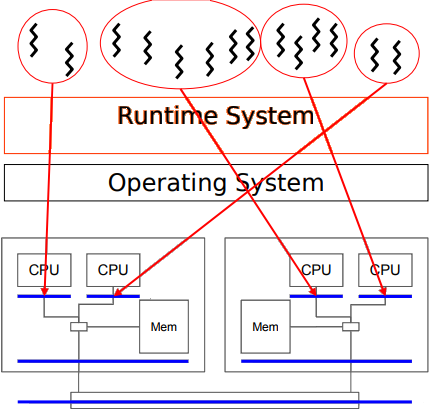
\includegraphics[scale=0.5]{bubbles001}
\centering
\caption{Principe de FORESTGOMP Framework}
\label{fig:mci7}
\end{figure}
%
\begin{center}%[htbp]
\begin{tabular}{l *{13}{l}} 		\hline
{TCH} & {IMP} 	& {SDP} 	&  {TSD} 	& {GRN} 	& {ToP} 	& {TYP} 	& {SPD}	& {ENT} 	& {ToS} \\     		\hline
C     	& OS		& PFL		&  - 		& PG		& EXE		& THD CLS	& OS 		& OS THD  & EXE  \\     		          \hline
\end{tabular}
 \captionof{table}{Caractéristiques de l'approche FORESTGOMP}% Add 'table' caption
\end{center}
%
\subsection{LAWS} %Task placement 	& Data distribution 	& Cilk tasks 	& Execution 	& x\\\lipsum 
%
\textbf{1- Auteurs}

Chen et al. \cite{Che38}

\textbf{2- Idée}

L'approche associe l'allocation et l'ordonnancement compatibles avec NUMA avec la programmation des tâches CILK. 
Elle cible les \textbf{algorithmes diviser pour régner} avec les caractéristiques suivantes: \\
a- les étapes récursives de l'algorithme sont représentées par un arbre de tâches dans lequel chaque nœud représente une étape.\\
b- les accès aux données ne se produisent que dans les tâches feuilles et le partage de données entre les tâches du même niveau dans l'arbre. 

LAWS a trois composants principaux: \\
i- un \textbf{allocateur de mémoire} compatible NUMA, \\
ii- un \textbf{packer DAG adaptatif}\\
iii- un \textbf{mécanisme de vol de travail} compatible avec NUMA et le cache. 

Son placement de données est effectué au cours de la première itération de l'algori-thme en affectant les ensembles de données des tâches crées de manière récursive de l'arbre de tâches aux nœuds NUMA.

\textbf{3- Expérimentation}

LAWS a été testé sur un système AMD Opteron 8380 à quatre nœuds exécutant un ensemble d'applications qui effectuent des \textbf{calculs de stencil} et des algorithmes pour l'\textbf{élimination gaussienne}. 
Chaque benchmark est disponible en deux versions. 
La première version a une exécution \textbf{DAG régulièrement structurée}, tandis que les calculs de la seconde version forment un \textbf{DAG de structure irrégulière}. 

\textbf{4- Evaluation}

La performance de LAWS a été comparée à CILK simple sans aucune modification et à un autre algorithme nommé CATS \cite{Che39}, qui n'adapte pas le placement après la première itération. 
L'amélioration de LAWS par rapport à CILK varie de 23:5\% à 54:2\%. 
LAWS surpasse systématiquement CATS, ce qui améliore les performances par rapport à CILK jusqu'à 19:6\%. 

\textbf{5- Commentaires}

LAWS montre que les informations implicites sur la structure des calculs ainsi que les structures de données impliquées dans les calculs peuvent être exploitées à la fois pour le placement de données et l'ordonnancement afin d'augmenter la localisation des accès mémoire automatiquement par le système d'exécution. 
%
\begin{center}%[htbp]
\begin{tabular}{l *{13}{l}} 		\hline
{TCH} & {IMP} 	& {SDP} 	&  {TSD} 	& {GRN} 	& {ToP} 	& {TYP} 	& {SPD}	& {ENT} 	& {ToS} \\     		\hline
C     	& RT		& DAG		&  ARY 	& BL		& EXE		& TSK		& DD 		& Cilk TSK 	& EXE  \\     		          \hline
\end{tabular}
 \captionof{table}{Caractéristiques de l'approche LAWS}% Add 'table' caption
\end{center}
%
Les tableaux 1.10 et 1.11 donnent un récapitulatif des caractéristiques principales pour toutes les approches présentées précédemment. 
%
\afterpage{
\clearpage% Flush earlier floats (otherwise order might not be correct)
\thispagestyle{empty}% empty page style (?)
\begin{landscape}
	\begin{center}%[htbp]

	\begin{tabular}{l *{13}{l}}
		\hline
	    	{Num} &     {Scheduling/Mapping Policy} &     {ONU} &     {OCH} &     {DPL} &     {SCH} &     {Impl layer} &     {DoRD} &  {Sup-DT} &     {Granularity} &     {ToD} &     {ADA} &    {Ref} \\
    		\hline
1		& Affinity on touch(OS)	& X 	& -		& X 	& - 	& LIB/OS		& PROGr 	& Any 			& PGs 			& EXE		& x 	& [61,50] \\
2         & CARREFOUR           		& X    	& -      & X     	& X     	& OS 			& PRFLg	& Any 			& PGs			& EXE		& x 	& [44] \\
3         & MAI                             & X    	& -      & X    	& -      	& LIB 			& PROGr 	& Arrays 		& BLs/PGs 		& EXE		& x 	& [77]\\
4         & MINAS + profiling         & X    	& X     	& X    	& (X)  	& PPg + LIB 	& PPr 		& Static Arrays & BLs/PGs 		& EXE		& x 	& [66,76] \\
5         & FBoPP 					& X    	& -      & X     	& -      	& LIB			& PRFLg 	& Any 			& PGs 			& EXE		& x 	& [62] \\
6         & SCHEDULE REUSE        & X    	& -      &(X)   	& X     	& CMPL+ RT	& PROGr 	& Arrays 		& ELTs			& EXE		& x 	& [68]\\
7         & Unstructured parallelism& - 		& X 	& - 	& X 	& RT			& - 		& - 			& - 			& EXE		& x 	& [86]\\
8       	& FORESTGOMP 			& X 	& X 	& X 	& X 	& RT			& PROGr 	& Not Specified& N/Specified	& EXE		& x 	& [29, 31]\\
9       	& LAWS 					& X 	& X 	& X 	& X 	& RT			& DAG 		& Arrays 		& BLs 			& EXE		& x 	& [38]\\
  		\hline
	\end{tabular}
	\label{table:TB_4_1_20}
	 \captionof{table}{Caractéristiques des approches et du placement de données associes}% Add 'table' caption

	\begin{tabular}{l *{8}{l}}
		\hline
		{Num} &     {Scheduling/Mapping Policy} &     {Type of placement} &     {Source for PLC decision} &     {Scheduling entity} &     {Time of decision} &     {Auto.dyn.adjustment}\\
		\hline
		1 		& Affinity on touch(OS)		& -    					& -      				& -     				& -      					& -\\
		2         & CARREFOUR                 	& Thread clustring   	& OS/PMU     		& OS threads     	& Execution     		& x\\
		3         & MAI                             	& Thread pinning    	& -      				& PThreads    		& Start of execution   	& -\\
		4         & MINAS + profiling              	& Co-scheduling    	& Data sharing     	& PThreads    		& Start of execution  	& -\\
		5         & Feedback-directed PLC 		& Thread pinning    	& -      				& PThreads     		& Start of execution    	& -\\
		6         & SCHEDULE REUSE            	& Loop scheduling   	& Data distribution & Loop iteration   	& Execution     		& -\\
		7         & Unstructured parallelism  	& Task placement 		& Data sharing 	& Tasks 			& Start of execution 	& x\\
		8        	& FORESTGOMP 			     & Thread placement	& Data distribution	& OpenMP threads	& Execution 			& x\\
		9         & LAWS 				     		& Task placement 		& Data distribution	& Cilk tasks 		& Execution 			& x\\
		\hline 
	\end{tabular}
	\label{table:TB_4_1_1}
	\captionof{table}{Caractéristiques de l'ordonnancement des approches vues}% Add 'table' caption
\end{center} 
\end{landscape}
\clearpage% Flush page
}
%===================================================================================
\newpage
\section{Stratégies d'équilibrage de charge dans NUMA}\label{straECNUMA}
%
L’algorithme d’ordonnancement dynamique doit être générique, évolutif et flexible sur la prise de décision. 
Cette flexibilité provient de la possibilité de choisir n’importe quelle tâche prête tout en conservant la borne sur le temps d’exécution.
Dans beaucoup d'algorithmes d'ordonnancement, l’objectif principal est de minimiser les temps d’inactivités et surtout cela lors de la communication. Pour aider à atteindre cet objectif, Les algorithmes de l'équilibrage de charge permettent de réduire cette inactivité en préservant une charge équitable entre les processeurs.

Chaque processeur maintient sa propre liste locale des tâches prêtes.
Cette commu-nication pourrait impliquer les transferts de données nécessaires pour compléter le travail, 
mais aussi les processeurs sont capables de communiquer pour échanger les tâches dans leurs files d'attente fonctionnelles. 
Le processus d'échange de tâches entre files d'attente est l'essence même de l'ordonnancement des algorithmes dynamiques. \cite{quint11}
Il existe deux grands paradigmes d'équilibrage de charge dynamique dans les plateformes parallèles NUMA inclus : \\
- Le partage de travail \cite{BL99}\\
- Le vol de travail \cite{BLU95}\\
%
\subsection{Partage du travail} 
%%Les processeurs partagent des tâches de leur liste prête aux listes prêtes d'autres processeurs. 
Dans la stratégie du partage de travail, chaque processeur a un ensemble de tâches à exécuter. 
Ce travail est enregistré dans la mémoire du processeur qui doit exécuter la tâche. 
Le risque est qu’un processeur ait plus de travail que les autres. 
Pour rééquilibrer la charge entre les processeurs, chaque processeur surveille sa quantité de travail . 
Si un processeur est surchargé, des tâches sont migrées vers les autres processeurs. 
Ainsi, les tâches sont échangées entre les processeurs pour équilibrer la charge.
Le choix de migration nécessite une méthode pour mesurer la quantité de travail totale et locale à un processeur, mais aussi le coût de la redistribution du travail. 
Au fur et à mesure de l’exécution, la quantité de travail diminue. 
Il est donc nécessaire de faire transiter des messages pour avoir les informations. 
Lorsque celles-ci sont connues, l’algorithme doit migrer les tâches afin d’obtenir un système dans lequel aucun processeur ne détectera de surcharge. \cite{quint11}

Pour les tâches homogènes et indépendantes, l’algorithme peut calculer la quantité de travail
sur toute la plate-forme et en local et il fonctionne bien dans ces conditions. 
En revanche, dans le cas général, cela implique des erreurs sur les temps d’exécution qui pourront être compensées par des migrations de tâches.
La prise en compte des relations de précédences et des coûts de communications entre les tâches compliquent sa tâche et demande d’importants changements dans l’algorithme. 
Dans ce cas, les migrations de tâches risquent d’être fréquentes pour compenser le manque d’informations.
Les performan-ces obtenues risquent d’être mauvaises. \cite{quint11}
%
\subsection{Vol de travail (Work stealing)}
%
Les processeurs tente de voler des tâches à partir de listes prêtes d'autres processeurs qui sont appelés \textbf{victimes (VICTIM)} lorsque sa propre file d'attente devient vide. 
Dans ce cas, ce processeur est appelé \textbf{voleur (THIEF)}, et la tâche volée migre vers la file d'attente de ce processeur en quittant celle du processeur volé \cite{SPO09}. 
Cet algorithme est implémenté dans certains langages comme Cilk \cite{BLU95}. 

L'objectif du vol de travail est de s’abstraire de toutes les données fournies par l’utilisateur tout en ordonnançant efficacement l’application sur un nombre de machines non défini. 
Ce mécanisme a été proposé initialement par Blumofe \cite{BLU95}.
Sa popularité provient de ses nombreux atouts, en voici  quelques un :\\
– algorithme distribué\\
– passage à l’échelle\\
– réactivité aux perturbations\\
– temps d’exécution et nombre de tâches transférées analysés théoriquement

%Une des principales propriétés du vol de travail est que l’algorithme est distribué.
Dans cet algorithme, les décisions sont généralement prises avec les informations locales à chaque processeur participant à l’exécution. 
Durant l’exécution, chaque processeur a une liste de tâches qui représente le travail à effectuer. 
Lors de l’exécution d’une tâche, le processeur exécute les instructions associées qui peuvent générer d’autres tâches. 
Ces tâches sont stockées pour la suite de l’exécution dans sa liste. 
L’ensemble des tâches et leurs données décrivent l’application qui est représentée par un DAG.
En fonction de la quantité de travail présente dans la liste, deux états sont distinguables pour les processeurs :
\\
- \textbf{Travailleur} ($NORMAL$) : un processeur qui exécute du travail (une tâche). Sa liste de tâches peut être vide ou non.\\
- \textbf{Victime} ($VICTIM$): un processeur qui exécute du travail (une tâche) et sa liste de tâches contient plus de tâches qu'un seuil fixé ($MAX\_TK$).\\
- \textbf{Voleur} ($THIEF$) : un processeur qui n’a plus de travail à exécuter. Sa liste de tâches est vide ou contient moins de tâches d'un seuil fixé ($MIN\_TK$).. 

Il tente de trouver du travail auprès des autres processeurs. 
Tous les processeurs évoluent entre ces trois états. 
Le passage de $THIEF$ à $NORMAL$ s’opère en demandant du travail aux autres processeurs. 
Si un processeur reçoit une demande de travail et s’il a des tâches dans sa pile, il envoie du travail au $THIEF$. 
Le passage de $NORMAL$ à $THIEF$ s’effectue en fonction des requêtes de vol et de l’exécution des tâches.
Dans ce mécanisme, l’ordre d’exécution des tâches est influencé par plusieurs décisions qui influencent énormément les performances du système : \\
1- la prochaine tâche à exécuter, \\
2- le processeur volé et la ou les tâches volées. \\
%
\subsubsection{Ordre d’exécution local}
%
L’ordre d’exécution est un des choix qui est le plus rarement modifié, car l’analyse théorique initialement réalisée par Blumofe et Leiserson \cite{BLU95},  montre que la décision de suivre le parcours initial du programme sans création de tâches (l’ordre séquentiel) est efficace. 
Le respect de l’ordre séquentiel permet de conserver les optimisations réalisées par le programmeur. 
De plus, ce choix permet de borner l’espace mémoire utilisé par chaque processeur. 
Cet espace mémoire est dans ce cas inférieur ou égal à l’espace mémoire utilisé par le programme séquentiel. 
Cet ordre d’exécution est équivalent à un parcours en profondeur du DAG de l’application. 
Au niveau de la liste, ce parcours peut être réalisé en sélectionnant la dernière tâche ajoutée ('Last In First Out (LIFO)').
%
\subsubsection{Requête de vol}
%
Lorsqu’un processeur devient $THIEF$, il choisit le processeur $VICTIM$ duquel il va prendre une partie du travail. 
Il existe un grand nombre de stratégies différentes. 
Une des stratégies pour le choix est simplement de réaliser un tirage aléatoire uniforme parmi les processeurs participant à l’exécution. 
Cette stratégie reste la plus simple, ne nécessitant aucune information avec un nombre de requêtes de vol borné.
Les analyses théoriques montrent qu’avec une telle sélection de la victime, la probabilité de sélectionner un processeur ayant une
quantité importante de travail est grande même avec un nombre limité de vols \cite{BLU95}.

Une autre stratégie qui choisit le processeur ayant la tâche la moins profonde dans sa pile.  
Cette solution minimise le temps d’exécution, mais elle nécessite de conserver une information du processeur possédant cette tâche sur toute la plateforme.
Pour prendre en compte l’influence des accès mémoires sur des plates-formes hiérarchiques ou non, des travaux ont montré qu’il est intéressant d’orienter les vols vers des tâches ayant des données qui pourront être accédées rapidement par $THIEF$. \cite{quint11}
%
\subsubsection{Réponse de vol}
%
Sur réception d’une requête de vol, un processeur doit sélectionner le travail à fournir.
L’algorithme réalisant la sélection du travail à transférer vers $THIEF$ s’exécute en concurrence du travail effectué par le processeur $VICTIM$. 
Classiquement dans le vol de travail, la dernière tâche ajoutée à la pile est la tâche sélectionnée pour être exécutée.
Ainsi, les processeurs accèdent à leur pile par le bas (ordre 'LIFO'). 
Pour ne pas perturber le travail de la victime, les tâches volées sont choisies prioritairement en haut de la pile (ordre 'FIFO'). 
Les conflits d’accès risquent d’apparaître uniquement quand le nombre de tâches est faible. 
Il reste à définir le nombre de tâches prises dans la pile. 
Lors d’un vol, l’objectif est d’équilibrer le travail entre les deux processeurs ($VICTIM$ et $THIEF$). 
Puisque $THIEF$ n’a pas assez de travail, la quantité de travail prise doit être proche de la moitié de celle présente sur la victime. 
%------------------------------------------------------------------------------------------
\newpage
\section{Conclusion}\label{concEdA}
%
Dans ce chapitre, nous avons exposé les différentes approches concernant l'ordon-nancement et le placement des tâches avec les données dans le contexte NUMA. 
Au début, nous avons caractérisé de façon générique les approches qui tentent d'assurer un de ces rôles de point de vue prise décision. Ces approches sont basées sur  certaines caractéristiques des architectures cibles et certaines informations à exploiter lors de son fonctionnement. En se basant sur ces caractéristiques, nous pouvons regrouper les approches en trois classes. la première qui focalise sur l'ordonnancement seulement, la deuxième sur le placement et la troisième combine les deux aspects.

Par la suite, nous avons présenté l'idée derrière chaque approche ainsi que son implémen-tation et son évaluation. A la fin de chaque section, nous avons commenté les avantages et les limites de l’approche étudiée. Cette démarche nous permet de comparer l'impact de l'intégration  de chaque approche sur les performances des systèmes NUMA. 

Comme l'équilibrage de charge est important pour préserver les performances, la dernière section a détaillé les stratégies utilisées pour cette fin en particulier celle du vol de travail qui nous intéresse par la suite.

Le chapitre suivant est dédié à présenter notre approche dont le principe est d'exploiter l'horizon d'exécution pour guider les processus d'ordonnancement et exposer une variante de vol de travail basé sur la distance NUMA.